 \documentclass[12pt,a4paper]{article}
\usepackage{amsmath}
\usepackage{amssymb}
\usepackage{epstopdf}
\usepackage{inputenc}
\usepackage{graphicx}
\usepackage{titletoc} 
\usepackage{fancyhdr}   
\usepackage[a4paper,pdftex]{geometry}	
\usepackage[english]{babel}
\usepackage{xcolor} 
\usepackage{enumerate}
\usepackage{fix-cm} 
\usepackage[notlof]{tocbibind}
\usepackage{amsmath}
\usepackage{listings}
\usepackage{float}
\usepackage{enumitem}
\usepackage{xcolor}
\usepackage{listings}
\definecolor{vgreen}{RGB}{104,180,104}
\definecolor{vblue}{RGB}{49,49,255}
\definecolor{vorange}{RGB}{255,143,102}
\renewcommand\lstlistingname{Appendix}
\renewcommand\lstlistlistingname{Appendix}

\makeatletter
\newcommand*\@lbracket{[}
\newcommand*\@rbracket{]}
\newcommand*\@colon{:}
\newcommand*\colorIndex{%
	\edef\@temp{\the\lst@token}%
	\ifx\@temp\@lbracket \color{black}%
	\else\ifx\@temp\@rbracket \color{black}%
	\else\ifx\@temp\@colon \color{black}%
	\else \color{vorange}%
	\fi\fi\fi
}
\makeatother

\usepackage{trace}

\usepackage{subcaption}
\begin{document}
	\begin{titlepage}
		\begin{center}
			
\includegraphics[scale=.4]{Figures/Cover}\\
			\vspace{1cm}
			\bf{ \large {Department of Computer Science and Technology} }
		\end{center}
		
		\vspace{4cm}
		\centering
		\textbf{\Huge Machine Learning}
		\vspace{.5cm}
		
		{\Large Homework 2}

		\vspace{4cm}
		
		\textbf{\LARGE Sahand Sabour}
		
		
		
		\vspace{0.5cm}
		
		{\large 2020280401}
		
		
		\vfill
		
	\end{titlepage}

	\section{DeepWalk}
	
	\subsection{Motivation}
	\noindent 
	
	\subsection{Methodology}
	\noindent 
	
	\subsection{Experiments}
	\noindent 
	
	\subsection{Personal Opinion}
	\noindent 
	
	\newpage
	\section{(GCN)}
	
	\subsection{Motivation}
	\noindent 
	
	\subsection{Methodology}
	\noindent 
	
	\subsection{Experiments}
	\noindent 
	
	\subsection{Personal Opinion}
	\noindent 
	
	\subsection{Comparison with DeepWalk}
	\noindent 
	
	\newpage
	\section{CogDL}
	
	\subsection{Testing CogDL Models}
	
	\noindent In this assignment, we are asked to run two models on two different datasets by running the provided scripts. The first script is as follows: python scripts/train.py --task unsupervised\_node\_classification -- dataset wikipedia --model deepwalk; by running this script, we would be training and testing the DeepWalk model on the Wikipedia dataset for the task of node classification. The results of this process is provided in the figure below (Figure 1).
	\begin{figure}[H]
		\centering
		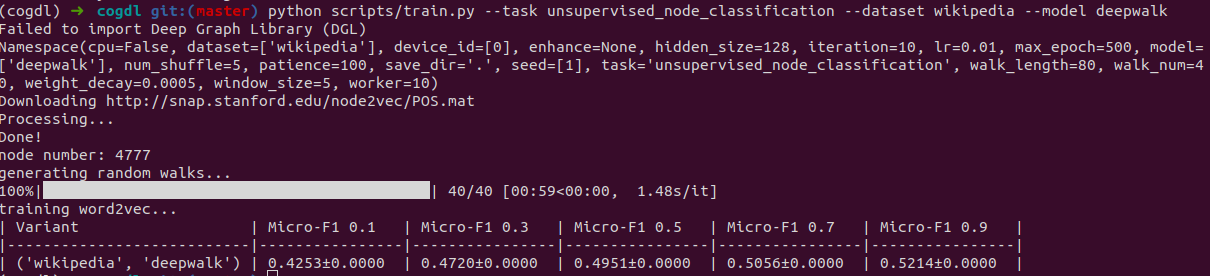
\includegraphics[width=15cm, height=5.5cm]{Figures/cmd1}
		\vspace{-0.7cm}
		\caption{Result of running the first script}
	\end{figure}

	\vspace{-0.4cm}
	\noindent Accordingly, the second script (python scripts/train.py --task node\_classification --dataset citeseer -- model gcn) analyzes the same task but for training and testing the GCN model on the citeseer dataset. The obtained results are demonstrated in the below figure (Figure 2).
	
	\begin{figure}[H]
		\centering
		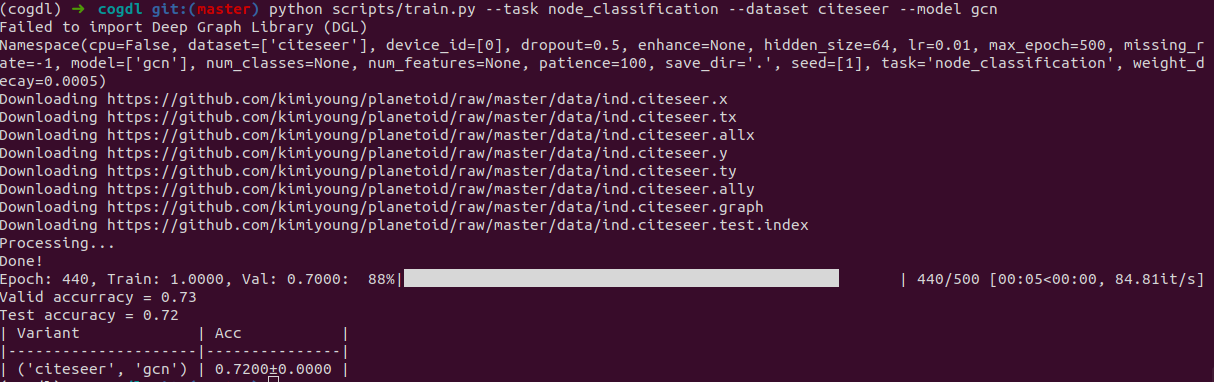
\includegraphics[width=15cm, height=6cm]{Figures/cmd2}
		\vspace{-0.7cm}
		\caption{Result of running the second script}
	\end{figure}
	
	\subsection{API Design}
	\noindent Similar to what is demonstrated in the two scripts of the previous section, the main entry point of the model training is train.py located in the scripts folder.
	
	\subsection{Implementation}
	
	\noindent In this assignment, I implemented the Hierarchical Graph Pooling with Structure Learning model [1]. The pull request id for this implementation is . 
	
	\subsection{Suggestions}
	\noindent There are a number of suggestions that I believe would improve the CogDL experience, both as a user and as a contributor:
	\begin{enumerate}
		\item hi
	\end{enumerate}
	
	\subsection{Contributions}
	
	\vspace{0.4cm}
	\section*{References}
	[1] Zhen Zhang et al. “Hierarchical graph pooling with structure learning”. In:arXiv(2019) arXiv:1911.05954


	
\end{document}